\documentclass[letterpaper,oneside,12pt]{article}
%\documentclass[letterpaper,oneside,12pt]{report}
\usepackage{graphicx}
\usepackage{rotating}
\usepackage[american]{babel}

\selectlanguage{american}

% page layout
%  \setlength{\hoffset}{-1in} 
  %\setlength{\voffset}{-1in}
%  \setlength{\textwidth}{15cm}
%  \setlength{\oddsidemargin}{3.5cm}
%  \setlength{\evensidemargin}{0.2cm}
%  %\setlength{\topmargin}{2.5cm}
%  \setlength{\headsep}{5ex}
%  \setlength{\textheight}{22cm}
%  \renewcommand{\baselinestretch}{1.05}
%  \raggedbottom
%  \newlength{\pictheight}
%  \setlength{\pictheight}{\textheight}
%  \addtolength{\pictheight}{-2cm}

% document
\begin{document}

%\begin{titlepage}
\hspace{-7mm}
\begin{minipage}{\textwidth}
\begin{center}
\vspace{.5cm}
{\huge \bf Software Design Document\\[1.5ex]}
{\large \bf for a specific implementation of `BCI2000'}
\\[1.5cm]
{\Large Gerwin Schalk\\}
{\Large Thilo Hinterberger\\}
{\Large Dennis J. McFarland\\[1.5cm]}
%
\begin{minipage}{13cm}
  \begin{minipage}[c]{13cm}
    \begin{center}
      {\Large \bf New York State Department of Health\\[2ex]}
      {\large \bf Wadsworth Center\\[0.5ex]
       Laboratory of Nervous Systems Disorders\\[4ex]}
      {\Large \bf Eberhard--Karls--Universit\"at T\"ubingen\\[2ex]}
      {\large \bf Medizinische Fakult\"at\\[0.5ex]
       Institut f\"ur Medizinische Psychologie\\[0.5ex]}
    \end{center}
  \end{minipage}
  \\[1.0cm]
  \begin{minipage}[c]{6cm}
    \centerline{
\includegraphics{figures/DOHlogo}}
  \end{minipage}
  \hspace{1.5cm}
  \begin{minipage}[c]{3cm}
    \centerline{
\includegraphics{figures/EKUlogo}}
  \end{minipage}
\end{minipage}
%
\\[0.5cm]
\textbf{Sponsors} \\
\textit{Jonathan R. Wolpaw and Niels Birbaumer}
\\[1.0cm]
{Albany, NY} \\[1ex]
{February 2000--May 2001}
\\[1ex]Updated May 2003, J\"urgen Mellinger
\end{center}
\end{minipage}
\end{titlepage}

\title{BCI2000-Compatible Audio-Visual P3 Task}
\author{Jennia Hizver, J\"{u}rgen Mellinger, Dennis McFarland, Gerwin Schalk}
\maketitle

\tableofcontents

\newpage 

\begin{abstract}

The main purpose of this task is to present a series of (auditory or visual) 
stimuli sequentially to the user of the BCI system. The sequence and nature of 
the stimuli can be defined by the investigator. In addition to stimulus 
delivery, the task can optionally be used in conjunction with BCI2000's P300 
Signal Processing module (P3SignalProcessing.exe) to provide feedback to a 
selected stimulus in either a copy or a free mode.

\end{abstract}

\section{Functionality}

\subsection{Stimulus Definition}
\label{sec:stimulusdefinition}

Stimuli are set up through a parameter defined by the application module. This
implicitly defines the total number of stimuli as well as the details of each stimulus.
Each stimulus is defined by the following properties:
\begin{enumerate}
 \item Caption
 \item Icon file
 \item Audio file
\end{enumerate}

In addition to stimuli, the parameter contains a definition for a stimulus that 
announces what to focus on, and a stimulus that announces the result. These
stimuli are only used when the task is set to copy or free mode.

The following table contains an example definition of two stimuli;
for clarity, the parameter line defining the associated parameter is also given:
\footnote{
  The line's parameter format contains to newly introduced extensions:
  \begin{itemize}
  \item In the place of a dimension value there may be a list of string labels
        that may be used instead of numerical indices, delimited by a matching
        pair of any of \{\},[],().
  \item A \texttt{\%} character followed by up to two hexadecimal digits represents
        a byte value in hexadecimal notation, thus \texttt{\%20} represents a
        space character, and \texttt{\%}, \texttt{\%0}, and \texttt{\%00} all
        represent an empty string value; \texttt{\%\%} represents the \texttt{\%}
        character itself.
  \end{itemize}
}

\begin{center}
\begin{tiny}
\begin{tabular}{r|llll}
           & focuson & result & stimulus1 & stimulus2 \\ \hline
   caption & Please focus on
           & The result was
           & Donkey
           & \\
      icon & \verb|icons\focus on.bmp|
           & \verb|icons\result.bmp|
           & \verb|icons\donkey.bmp|
           & \verb|icons\elefant.bmp|\\
     audio & \verb|wav\focus on.wav|
           & \verb|wav\result.wav|
           & \verb|wav\snicker.wav|
           & \verb|wav\trumpet.wav|\\	
\end{tabular}
\end{tiny}
\end{center}
\label{tab:stimuli_example}

\begin{verbatim}
"P3AV matrix Stimuli= "
      "{caption icon audio} "                  // row labels
      "{focuson result stimulus1 stimulus2} "  // column labels
      
      // focuson
      "Please%20focus%20on icons\\focus%20on.bmp wav\\focus%20on.wav "
      // result
      "The%20result%20was icons\\result.bmp wav\\result.wav "
      // stimulus1
      "Donkey icons\\donkey.bmp wav\\snicker.wav "
      // stimulus2
      "% icons\\elefant.bmp wav\\trumpet.wav "
\end{verbatim}

\emph{Comments:} The stimulus properties might contain white spaces. A 
caption/icon/audio file are not being presented, if they are not defined (e.g., 
see caption in stimulus2). The stimulus definition parameter does \emph{not} contain 
a description on how the stimuli are presented. Stimulus numbers start at 1.
Relative paths are interpreted relative to the application module's executable
location.\footnote{Which, in general, is not the application module's
working directory at runtime but the path portion of the first argument to \texttt{main()}.}

\subsection{Stimulus Sequence}

Stimuli are presented in a certain sequence. This sequence can either be 
deterministic, i.e., defined by the investigator, or random. 

\subsubsection{Deterministic Sequence:}The investigator defines the order by 
entering a list of stimulus IDs to be presented. As an example: 
\begin{verbatim} 
1 5 3 4 2 
\end{verbatim} 
defines a sequence in which stimulus 1 is first presented, followed by 
stimulus 5, etc.

\subsubsection{Random Sequence:}The investigator defines absolute stimulus 
frequencies for each stimulus, with the sum $N$ of those values equaling the total
number of stimulus presentations in the final sequence. The resulting random
sequence is obtained by applying a random permutation to an arbitrary sequence
that reproduces the given frequencies, with all $N!$ index permutations being
equally probable (Block Randomization).
\footnote{Block randomization routines, as well as a pseudo random generator better
than the one available via \texttt{rand()}, are available in the P3 Speller module.}

As an example: 
\begin{verbatim} 
6 2 3
\end{verbatim} 
defines a sequence of 11 stimulus presentations with stimulus 1 being presented 6
times, stimulus 2 2 times, and stimulus 3 3 times. The resulting sequence $S_1$ will
be a permutation of $S_0 = [1, 1, 1, 1, 1, 1, 2, 2, 3, 3, 3]$, and the probability
for $S_1$ to equal $S_0$ will be
$\frac{6!\times2!\times3!}{(6+2+3)!}=1/4620$.

Multiple sequences can be generated from the given frequencies.
The investigator can define how many sequences are generated and played.

\subsection{Stimulus Delivery}

For any stimulus, delivery occurs simultaneously for caption\footnote{A caption, 
if defined, always appears in front on an icon.}, icon, and audio. (A computer 
can only execute commands in sequence, but the time difference between start of 
presentation of caption, icon, and audio, is negligible). \emph{Comment:} A 
knowledgeable investigator has to understand the implications of audio files 
that are of unequal length !

An investigator can specify:
\begin{itemize}
 \item Size and position of the target window (using the same scheme/parameters 
       as used by the RJB task, Oddball paradigm, or P3 speller).
 \item Width and height of caption and icon in percent of screen
       width/height\footnote{Using, e.g., the \texttt{TImage::Stretch} property for scaling.}
 \item Whether captions, icons, or audio files will be presented
       (i.e., a global switch). There are no individual switches for each stimulus. However,
       captions/icons/wave files will not be presented for individual stimuli if they are not defined (i.e., their respective entries are blank).
 \item The volume for audio playback as a float value between 0 and 1
 \item Window background color in RGB\footnote{For convenience, RGB values
       may be entered in hexadecimal notation, e.g. \texttt{0xff0000} for red.}
 \item Caption color in RGB
 \item The duration during which a stimulus is presented (in units of
       SampleBlocks)\footnote{Playback of audio extending above the specified duration 
       will be muted.}
 \item The duration of an inter-stimulus interval following stimulus presentation
       (in units of SampleBlocks)\footnote{During the inter-stimulus interval, the
       screen is blank and audio is turned off.}
 \item A minimum and maximum time (in units of SampleBlocks) that will be added randomly
       to the inter-stimulus interval, with probability distributed uniformly over time
       intervals.
       If these variables are both set to 0, the actual inter-stimulus interval will
       always be exactly as defined above.
       If these variables are set to, for example, 0 and 3, inter-stimulus intervals
       will randomly be longer by between 0 and 3 units, with a probability of $1/4$
       for the occurrence of any one of the four time intervals possible.
 \item A Comment. A user can enter comments to the specific run in a string parameter.
\end{itemize}


\section{Processing of Classification Results}

The task can be configured to interpret results communicated to it by the P3 
Signal Processing module. These results represent a judgment on which of the 
stimuli was most likely selected. Handling of these results is identical to the 
P3 Spelling Task. 

When it transmits a classification result, Signal Processing sets the state 
\emph{StimulusCodeRes} to the stimulus code that was originally transmitted to 
it by the user application. For example, when it sets \emph{StimulusCodeRes} to 
3, it indicates that it transmits classification results for stimulus 3. In 
addition, it sets \emph{StimulusTypeRes} to reflect the type of the stimulus 
(0=non-target, 1=target) when the system is in copy mode. Signal Processing 
transmits the classication result as one number (i.e., the first control signal).

\subsection{Free Mode}

The task can be configured to operate in free mode. In this case, the sequence 
of stimulus delivery is followed by a time period, in which the result of Signal 
Processing's classification is announced. The final classification result is
the stimulus with the highest classification result.

In order to deliver this announcement, the system uses the stimulus defined in 
the \texttt{result} column of the stimuli parameter. This announcement is 
followed by delivery of the determined stimulus. In other words, after a 
sequence of stimulus delivery, the system might play a .wav file that says: "the 
result is," followed by a .wav file that says "yes." (assuming "yes" represents
the stimulus that produced the highest classification result).

Finally, the task sends this result to the operator module as an ASCII text 
message so that it appears in a log window.

Free mode does not terminate until the investigator suspends operation.


\subsection{Copy Mode}

Copy mode is similar to free mode. In copy mode, the investigator can define a 
list of stimuli to be copied (e.g., "3 5 4"). In this example, the user has to 
attend to stimulus 3 for the first sequence, 5 for the second sequence, etc.

In addition to an announcement of the result, in copy mode the delivery of 
stimuli is preceded by an announcement that describes which stimulus the user
has to attend to. This announcement uses the stimulus that is defined in the
\texttt{focuson} column of the stimuli parameter. This announcement is followed by
delivery of the desired target stimulus. As an example, the system might say
"Please focus now on" ... "yes," before it starts with the sequence of
stimulus delivery.

Copy mode terminates (i.e., the task suspends) when the user finished copying 
all stimuli specified by the investigator.

\section{Parameters}
The following parameters configure this task:
\begin{itemize}
 \item {\tt WinXpos, WinYpos, WinWidth, WinHeight}: Size and position of the target window (using the same scheme/parameters 
       as used by the RJB task, Oddball paradigm, or P3 speller).
 \item {\tt WinBackgroundColor}: Window background color in RGB\footnote{For convenience, RGB values
       may be entered in hexadecimal notation, e.g. \texttt{0xff0000} for red.}
 \item {\tt StimulusWidth}: Width of stimulus in percent of screen. Height is deduced based on the respective icon's aspect ratio.
 \item {\tt AudioSwitch}: Whether audio files will be presented
       (i.e., a global switch). There are no individual switches for each stimulus. However,
       wave files will not be presented for individual stimuli if they are not defined. The values can be: 0(off) and 1(on).
 \item {\tt VideoSwitch}: Whether video files will be presented
       (i.e., a global switch). There are no individual switches for each stimulus. However,
       icons files will not be presented for individual stimuli if they are not defined. The values can be: 0(off) and 1(on).
 \item {\tt CaptionSwitch}: Whether captions will be presented
       (i.e., a global switch). There are no individual switches for each stimulus. However,
       captions will not be presented for individual stimuli if they are not defined. The values can be: 0(off) and 1(on).
 \item {\tt AudioVolume}: The volume for audio playback as a float value between 0 and 1
 \item {\tt CaptionColor}: Color of stimulus caption text in hex (0x00BBGGRR).
 \item {\tt CaptionHeight}: Height of stimulus caption text in percent of screen.
 \item {\tt OnTime}: The duration during which a stimulus is presented (in units of
       SampleBlocks)\footnote{Playback of audio extending above the specified duration 
       will be muted.} The way it translates to seconds is {\tt OnTime} multiplied by {\tt SampleBlockSize}(samples transmitted per time) divided by {\tt SamplingRate}(samples per one second).
 \item {\tt OffTime}: The duration of an inter-stimulus interval following stimulus presentation
       (in units of SampleBlocks)\footnote{During the inter-stimulus interval, the
       screen is blank and audio is turned off.}
 \item {\tt MinInterTime, MaxInterTime}: A minimum and maximum time (in units of SampleBlocks) that will be added randomly
       to the inter-stimulus interval, with probability distributed uniformly over time
       intervals.
       If these variables are both set to 0, the actual inter-stimulus interval will
       always be exactly as defined above.
       If these variables are set to, for example, 0 and 3, inter-stimulus intervals
       will randomly be longer by between 0 and 3 units, with a probability of $1/4$
       for the occurrence of any one of the four time intervals possible.
 \item {\tt PreSequenceTime}: The duration(in SampleBlocks) before a sequence is presented. During this time the following is going to happen. In Copy Mode: "Please, focus on ..." message will be played followed by the actual stimulus that the subject needs to focus on.
 In Free Mode and No-Interpretation Mode: during this time nothing will be presented, just a plain blank screen.
 \item {\tt PostSequenceTime}: The duration(in SampleBlocks) after a sequence is presented. During this time the following is going to happen. In Copy Mode and Free Mode: "The result was ..." message will be played followed by the predicted stimulus.
 In No-Interpretation Mode: during this time nothing will be presented, just a plain blank screen.
 \item {\tt Matrix}: Defines all the possible stimuli which can be presented on the screen. See description in \ref{sec:stimulusdefinition} section.
 \item {\tt FocusOn}: Defines a stimulus that is used to announce "please, focus on .." message.
 \item {\tt Result}: Defines a stimulus that is used to announce "the result is .." message.
 \item {\tt Sequence}: Sequence of stimuli that is presented to the user (deterministic type) / Frequencies for for each stimulus (random sequence).
 Stimuli are defined as column indices into the  {\tt Matrix } parameter.
 \item {\tt SequenceType}: Specifies whether the sequence is deterministic (value 0) or random (value 1).
 \item {\tt NumberOfSeq}: Number of sequences being presented to the user in a single run.
 \item {\tt InterpretMode}: None(value 0, no interpretation)/Free(value 1)/Copy(value 2) mode. If interpretation mode is set to none, the task does not rely on presence of 
 {\tt StimulusCodeRes} and {\tt StimulusTypeRes} states and thus can be used with other signal processing modules.
 \item {\tt ToBeCopied}: A list of stimuli that user needs to copy (only in copy mode). 
 \item {\tt UserComment}: A Comment. A user can enter comments to the specific run in a string parameter.
\end{itemize}

The following conditions need to be satisfied: 
\begin{itemize}
  \item Sound card has to be present if wave files are defined and global audio switch is on.
  \item All the parameters have to be present.
  \item {\tt MinInterTime} has to be less than {\tt MaxInterTime}.
  \item {\tt PreSequenceTime} and {\tt PostSequenceTime} have to be at least 2 times larger than {\tt OnTime}. This follows from the fact
  	that during presequence and postsequence there will be 2 stimuli presented: one is for "please, focus on .."/"the result is .." and the
  	other for the actual name of the stimulus.		
  \item The time defined by {\tt PostSequenceTime} multiplied by {\tt SampleBlockSize} has to be larger than the value defined by {\tt NumSamplesInERP}.
\end{itemize}



\section{States}

The time line of stimulus delivery is encoded in state variables as defined in
Table~\ref{tab:states}.
\begin{table}
\begin{center}
\begin{tabular}[ht]{|l|l|l|}
\hline
\bf{State Name}& \bf{Bits}            & \bf{Description} \\
\hline
\hline
 SelectedStimulus & 7 & stimulus ID of finally selected stimulus \\
                  &   & only $>$0 when determining selected stimulus\\
\hline
 PhaseInSequence  & 2 & 0 in inter-stimulus interval\\
                  &   & 1 period prior to stimulus sequence (if any)\\
                  &   & 2 stimulus sequence period\\
                  &   & 3 period after stimulus sequence (if any)\\
\hline
 StimulusTime     & 16& time in ms as calculated in P3 Speller\\
\hline
 StimulusCode     & 7 & stimulus ID of currently visible stimulus\\
                  &   & or 0 if no stimulus visible\\
\hline
 StimulusType     & 1 & 0 in free mode; copy mode :\\
                  &   & 1 when current stimulus equals target stimulus\\
                  &   & 0 otherwise\\
\hline
 Flashing         & 1 & 1 during stimulus presentation, 0 otherwise\\
\hline
\end{tabular}
\caption{Encoding scheme for this task.}
\label{tab:states}
\end{center}
\end{table}

\section{Time line}

\begin{figure}[ht]
 \centerline{\scalebox{1}{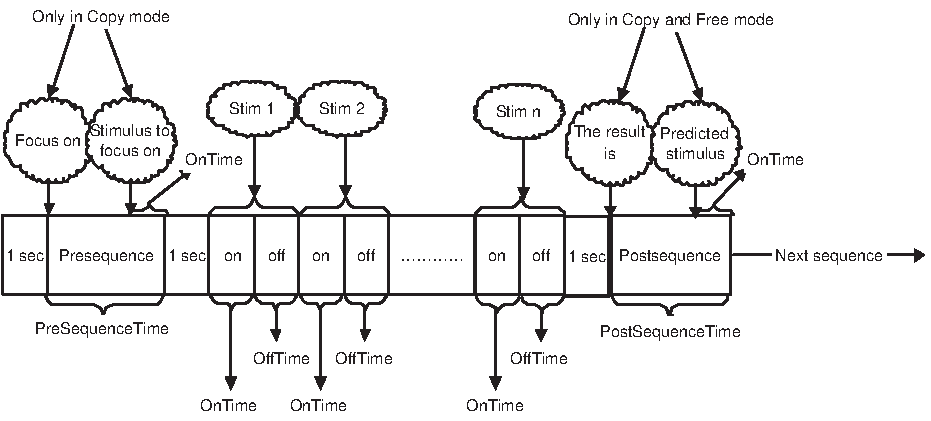
\includegraphics{TimeLine.pdf}}}
 \caption{Time line.}
 \label{fig:timeline}
\end{figure}

%\appendix

\end{document}

